% Finished September 11, 2013
% Put into VUW Thesis format Wednesday 2 April 2014

\documentclass[12pt, a4paper, twoside, openright]{book}

\usepackage{vuwthesis} % sets up some local things, mostly the front page

\setlength{\intextsep}{12pt} % set space above and below in-line float
\setlength{\abovecaptionskip}{0pt} % set space between figure and caption.

\usepackage{url}

\usepackage{amssymb, amsmath}
%\usepackage{mathtools}
\usepackage{tikz}
\usetikzlibrary{calc}

\newcommand{\beff}{\ensuremath{b_{\mathrm{eff}}}}
\newcommand{\bmin}{\ensuremath{b_{\mathrm{min}}}}
\newcommand{\bmax}{\ensuremath{b_{\mathrm{max}}}}
\newcommand{\bfar}{\ensuremath{b_{\mathrm{far}}}}

%\usepackage{marvosym}

\usepackage{etoolbox}
\newtoggle{compilealone}
\toggletrue{compilealone}

\title{Chapter 8: Numerical Testing}
\author{Nat Lund}

\begin{document}
\chapter{Numerical Testing}\label{C:numerics}

We have derived an analytic formula for the effective slip length of a mixed slip surface, using two different mathematical techniques.  The expression is an approximation that becomes more and more exact as the limit of vanishing surface period is approached.  We expect the formula to be useful if the the physical system is `near the limit'.
We cannot precisely quantify `nearness to the limit': In our model we have two length scales, the period of slip variation $L$, and the minimum slip length $\bmin$, and our formula is exact in the limit $L \to 0$.  All we can say is that a system is `near the limit' if $L$ is `near to 0' \emph{compared to $\bmin$.} That is, a system is near the limit if $L \ll \bmin$.

Our formula predicts an effective slip length; we wish to test our prediction against the `true' slip length. In particular, we wish to compare our prediction with the true slip lengths of systems as they move ever further from the limit.  The only true effective slip length is one measured in a physical experiment.  Such experiments are beyond the scope of this thesis.  However, the next best thing is a computer experiment, usually referred to as a numerical simulation.

\section{Finite Element Modeling}

Perhaps the most powerful and versatile numerical method for solving partial differential equations is Finite Element Modelling (FEM).  Many industrial-strength implementations are available; we chose the free and open-source package \textbf{FreeFem++}, available from \url{www.freefem.org}.

Using FreeFem++, we modeled a two-dimensional fluid driven by a fixed shear rate of 1 at the top boundary.  The slip boundary at the bottom was a sine wave profile, with an intrinsic slip length that varied in a binary fashion with the same period: The slip length on the peak of the sine wave was a low value, and the slip length on the trough of the sine wave was a high value.  This models shear-driven flow transverse to a grating or corrugation, with an air pocket in the grooves. 
A schematic is shown in Figure (\ref{FEMmodel}).


\begin{figure}[ht]
\centering
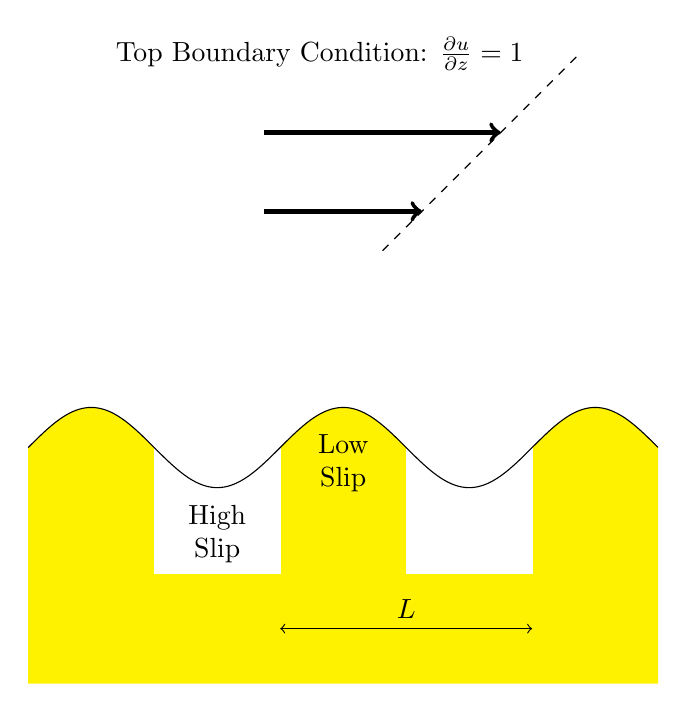
\begin{tikzpicture}
\node at (3.7,5) {Top Boundary Condition: $\frac{\partial u}{\partial z} = 1 $};

\draw[->, ultra thick] (3,4) -- ++(3,0);
\draw[->, ultra thick] (3,3) -- ++(2,0);
\draw[dashed] (3,2.5) ++(1.5,0) -- ++(2.5,2.5);

% \L = 3.2; length of period
\fill [color=yellow,domain=0:8,samples=200] plot (\x,{ (3.2 /6.2823) * sin( 6.2832 *\x / 3.2 r)} ) -- ++(0,-3) -| (0,0);

\draw[color=white,fill=white] (1.6,0) rectangle ++(1.6,-1.6);
\draw[color=white,fill=white] (4.8,0) rectangle ++(1.6,-1.6);

\draw [domain=0:8,samples=200] plot (\x,{ (3.2 /6.2823) * sin( 6.2832 *\x / 3.2 r)} );

\draw[<->] (3.2,-2.3) -- node[above] {$L$} ++(3.2,0);

\renewcommand{\baselinestretch}{1.00}
\node at (2.4,-1.1) [align=center] {High \\ Slip};
\node at (4,-0.2) [align=center] {Low\\ Slip};


\end{tikzpicture}
\caption{Schematic of the model used in the finite element analysis.}\label{FEMmodel}
\end{figure}

\clearpage
The FEM analysis was done for a series of sinusoidal slip surfaces, each with a different period $L$, but with the same intrinsic slip length values.  The FEM solution for each surface is a velocity field; from the far-field part of this solution an effective slip length $\bfar$ was calculated.  The fixed slip lengths and the sine wave profile were plugged into our formula, generating $\beff$.  The results are plotted in Figure (\ref{FEMplot}).  The solid line is the predicted $\beff$ (which does not depend on $L$), and the dots are the simulated $\bfar$ values at various values of $L$.


\begin{figure}[ht]
\includegraphics[scale=0.595]{Lund_Thesis_FEM_plot}
% Absurd scale factor is to suppress the error message!
\caption{Dots are values of $\bfar$ -- the effective slip length values calculated from the far-field velocity solutions of FEM simulations.  Solid line is the predicted $\beff$.  Dotted line is the $\beff$ predicted if the surface were assumed to be flat. }\label{FEMplot}
\end{figure}


As noted, a system is `near to the limit' if $L \ll \bmin$, in which case the predicted $\beff$ should approximate measured $\bfar$ very well.  This is true.  At $L = 0.1 \bmin$, the plot shows the numerically-calculated $\bfar$ (dots) to be within a few percent of predicted $\beff$ (solid line).

For interest,
the dashed green line is the effective slip length calculated if the surface were naively assumed to be flat.  Comparison with the numerical values shows the importance of the correction from using true contact area: the naive flat calculation overshoots numerical slip lengths by about 20\%.



But the pleasant surprise is that our full roughness-corrected $\beff$ prediction appears to be good even where $L \sim \bmin$.
For ease of comparing relative magnitudes, in Figure (\ref{FEMplotpcnt}) we plot the data with $\bfar$ expressed as a percentage difference from $\beff$.


\begin{figure}[ht]
\includegraphics[scale=0.595]{Lund_Thesis_FEM_plot_pcnt}
% Absurd scale factor is to suppress the error message!
\caption{Triangles are values of $\bfar$ -- effective slip lengths from FEM simulations.  Solid line is predicted $\beff$.  Dashed lines are 5\% above and below $\beff$.}\label{FEMplotpcnt}
\end{figure}

We see that if $L \leq \bmin$, then the numerical results differ from our prediction by less than 5\%.

So, while \emph{a priori} we can only expect our prediction to be trustworthy if $L \ll \bmin$, in practice --- or at least in this numerical simulation --- our prediction is very good for much larger values of roughness period, where $L \leq \bmin$.


\vspace{2em}

A final note about numerical issues:  A close look look at the data plotted above reveals that the numerics and the prediction agree better and better as $L$ gets smaller and smaller --- up to a point.  Then the prediction \emph{underestimates} the numerical values.  We believe this to be a computational artefact.  As the simulations were tuned, using finer and finer mesh granularity, in the regime $L \ll \bmin$, the $\bfar$ values got closer and closer to predicted $\beff$ (overshooting by less and less).  Extrapolating to the limit of infinite computing power, we believe the numerics would \emph{never} overshoot $\beff$, and the overshoot seen here is due to an insufficient number of lattice points on a very small and rapidly oscillating sine wave boundary.


\clearpage
\section{Finite Difference Numerics}

As an exercise, the same slip problem was also solved numerically using the finite difference method.  This was implemented in Python using the Numpy library, which is a front end to various very fast C and Fortran libraries.  A curved boundary is difficult to implement in this approach, so the case of the flat slip boundary was studied.

The main benefit of this exercise was the easy visualisation of the flow fields. Three-dimensional velocity profiles were generated.  The $x$-velocity $u$ for flow over a mixed-slip surface is shown in Figure (\ref{flow}).


\begin{figure}[ht]
\centering
\begin{tikzpicture}
\node [above right] { \includegraphics[scale=0.595]{Lund_Thesis_Flow} };

\coordinate (origin) at (4.53,0.22);
\draw[->] (origin) -- node[below]{$x$} ++(11:3cm);
\draw[->] (origin) -- node[below]{$z$} ++(150:2.5cm) -- node[left]{$u$} ++(0,5);
\draw (origin) ++(150:2.5cm) ++(0,4.17) -- ++(-0.15,0) node[left] {$u_P$};

\node at (6.8,1.65)[right]{$u$ with mixed-slip boundary};
\end{tikzpicture}
\caption{The coloured surface is $u$, the $x$-velocity component of a velocity field of a finite difference simulation of flow over a flat mixed-slip surface.}\label{flow}
\end{figure}


The $x$-velocity is high and uniform at the top boundary condition (large $z$), and varies periodically over the slip boundary.

\clearpage
To provide some perspective, flow profiles over \emph{pure} high-slip and low-surfaces were generated.  These are plotted together, along with the mixed-slip flow profile, in Figure (\ref{flowhilo}).

\begin{figure}[ht]
\centering
\begin{tikzpicture}
\node [above right] { \includegraphics[scale=0.595]{Lund_Thesis_Flow_HiLo} };

\coordinate (origin) at (4.53,0.22);
\draw[->] (origin) -- node[below]{$x$} ++(11:3cm);
\draw[->] (origin) -- node[below]{$z$} ++(150:2.5cm) -- node[left]{$u$} ++(0,5);
\draw (origin) ++(150:2.5cm) ++(0,4.15) -- ++(-0.15,0) node[left] {$u_d$};

\node at (6.6,2.7)[right]{$u$ with high-slip boundary};
\node at (6.6,1.8)[right]{$u$ with mixed-slip boundary};
\node at (6.6,1.25)[right]{$u$ with low-slip boundary};

\end{tikzpicture}
\caption{The same mixed-slip flow field as in Figure (\ref{flow}), plus the flow solutions for flow over the purely high-slip surface (pink), and the purely low-slip surface (yellow).}\label{flowhilo}
\end{figure}

There is an interesting feature in the mixed-slip flow field: while the velocity at the slip boundary varies periodically, the variation is not very large.  The slip velocity does \emph{not} swing between the extremes of velocities over the pure high-slip and low-slip surfaces.  Instead, the slip velocity has only a moderate periodic variation about a central value.

What is that central value?  Of course, we expect it to be the slip velocity that would occur if the surface had a single slip length equal to our predicted $\beff$.
We explore this by generating a last flow profile with a pure $\beff$ slip length surface.  We plot this (in black) together with the mixed-slip flow profile in Figure (\ref{floweff}).

\clearpage
\begin{figure}[ht]
\centering
\begin{tikzpicture}
\node [above right] { \includegraphics[scale=0.595]{Lund_Thesis_Flow_Eff} };

\coordinate (origin) at (4.53,0.22);
\draw[->] (origin) -- node[below]{$x$} ++(11:3cm);
\draw[->] (origin) -- node[below]{$z$} ++(150:2.5cm) -- node[left]{$u$} ++(0,5);
\draw (origin) ++(150:2.5cm) ++(0,4.17) -- ++(-0.15,0) node[left] {$u_d$};

\node at (6.7,1.9)[right]{$u$ with $\beff$ slip boundary (black)};
\node at (6.6,1.45)[right]{$u$ with mixed-slip boundary};
\end{tikzpicture}
\caption{The same mixed-slip flow field as in Figure (\ref{flow}), plus the flow field corresponding to a homogeneous boundary of slip length $\beff$ (black).}\label{floweff}
\end{figure}

This shows stunning agreement between the effective flow profile and the mixed-slip profile.  For most of the domain, they are almost indistinguishable.  Only very close to the slip boundary does the mixed-slip profile exhibit a periodic variation about the effective slip profile.

\vspace{1em}

This last plot also throws light on another issue: how thick is the boundary layer?  The boundary layer can be  arbitrarily defined to end where the flow becomes (arbitrarily close to) uniform.  Without being quantitative, we can see that a reasonable choice for boundary layer thickness $d$ could be less than the period $L$.
%  This would explain why the FEM simulations showed that $\beff$ works unexpectedly well even when it is not strictly true that $L \ll \bmin$.  The explanation is that even when $L \sim \bmin$, it may still be true that $d < \bmin$.  

%Finally, recall that the condition $L \ll \bmin$ is not a `requirement' as such.  In the mathematical model, $L$ and $\bmin$ are the appropriate nonarbitrary length scales, and the expression for $\beff$ becomes more and more exact as $L \to 0$.  To summarise the concept `$L$ is closer to zero than $\bmin$ is close to zero', one simply states that $L \ll \bmin$.

\iftoggle{compilealone}
    {
    \bibliography{Lund_Thesis.bib}
    \bibliographystyle{plain}
    }

\end{document}
